
% This LaTeX was auto-generated from MATLAB code.
% To make changes, update the MATLAB code and republish this document.

\documentclass{article}
\usepackage{graphicx}
\usepackage{color}

\sloppy
\definecolor{lightgray}{gray}{0.5}
\setlength{\parindent}{0pt}

\begin{document}

    
    
\subsection*{Contents}

\begin{itemize}
\setlength{\itemsep}{-1ex}
   \item derivatives
   \item Phase portrait
   \item function to evaluate derivatives in a mesh
\end{itemize}
\begin{verbatim}
clear; close all;
\end{verbatim}


\subsection*{derivatives}

\begin{verbatim}
f1 = @(x1,x2)(-x1 - x2/log(sqrt(x1^2+x2^2)));
f2 = @(x1,x2)(-x2 + x1/log(sqrt(x1^2+x2^2)));
\end{verbatim}


\subsection*{Phase portrait}

\begin{verbatim}
lim = 2; N = 21;
[X,Y,U,V] = derivatives(lim,N,f1,f2);
% Use quiver to plot; S = 0.75 to ensure arrows don't intersect
figure;
quiver(X,Y,U,V,0.5);
xlabel('x_1'); ylabel('x_2');
title('Phase portrait Q7');
\end{verbatim}


\subsection*{function to evaluate derivatives in a mesh}

\begin{verbatim}
function [X,Y,U,V] = derivatives(lim,N,f1,f2)
    % ---------------------------------------------------------------------
    % function to generate derivatives
    % lim - limits of the x,y grid of the plot. derivatives will be
    % evaluated at points between -lim to +lim
    %
    % N - number of points on each axis
    %
    % f1 - x derivative (xdot)
    % f2 - y derivative (ydot)
    % ---------------------------------------------------------------------
    % Generate mesh
    x = linspace(-lim,lim,N);
    y = linspace(-lim,lim,N);
    [X,Y] = meshgrid(x,y);
    % Variables to store derivatives
    U = zeros(size(X));
    V = zeros(size(X));
    for i = 1:length(X)
        for j = 1:length(Y)
            % Evaluate the derivatives
            u = f1(X(i,j),Y(i,j));
            v = f2(X(i,j),Y(i,j));
            r = sqrt(u^2+v^2);
            % Normalizing them to 1 and storing
            U(i,j) = u/r;
            V(i,j) = v/r;
        end
    end
end
\end{verbatim}

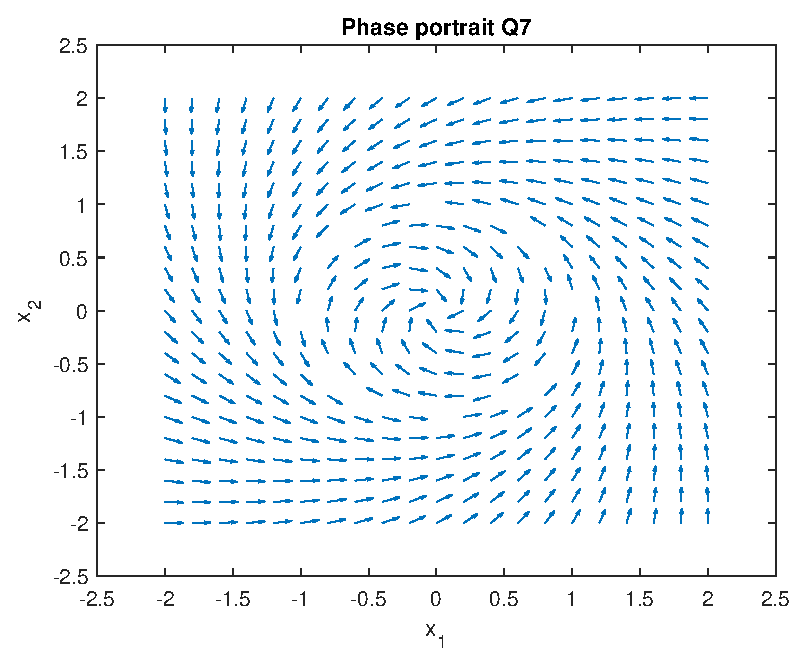
\includegraphics [width=4in]{Q7_01.eps}



\end{document}

